\section{Evaluation}\label{s:eval}

\begin{figure}
    \centering
\begin{knitrout}
\definecolor{shadecolor}{rgb}{0.969, 0.969, 0.969}\color{fgcolor}
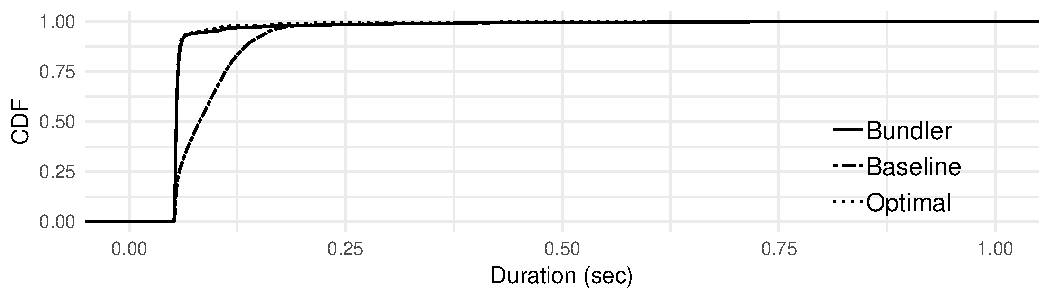
\includegraphics[width=\maxwidth]{figure/eval:best-1} 

\end{knitrout}
    \caption{\name achieves $33$\% lower median slowdown. Note the differing axis scales. For both \name and Optimal, performance benefits come from preventing short flows from queueing behind long ones. \an{Whiskers currently show 1.25 inter-quantile range, figure out how to show 99th \%ile? Also, can barely see Bundler and Optimal...}}
    \label{fig:eval:best}
\end{figure}


\begin{outline}[enumerate]
    \1 Bundler can reduce flow completion times
        \2 Base case with no cross traffic: run empirical traffic generator in the bundle varying offered load from 30\% to 90\%
            \3 Rough estimate of current results: 2-3x better for short flows (normalized fct, and only 10-20\% worse for long flows
            \3 Run with and without FQ scheduling, should still see some benefit from scheduling at lower load since there will be spikes of larger flows
            \3 Show how close bundler is to ideal situation (bottleneck router doing FQ scheduling) without actually having to change the middle of the network
        \2 Add inelastic background traffic
        \2 Add elastic background traffic
            \3 Have to enable x-tcp mode (perhaps dynamic number of flows) for bundler
            \3 can measure number of flows by looking at the number of backlogged queues
    \1 Microbenchmarks
        \2 Show that the bundler architecture is capable of emulating rate-based congestion control algorithms: \textbf{PLOT} throughput and delay of Nimbus/BBR/etc with and without bundler show that they look the same and achieve the same average behavior 
            \3 Regardless of underlying number of flows
        \2 Show that the measurements obtained via packet sampling are robust even though epoch size is varying over time due to hashing
        \2 Show why dynamic epoch adjustment is needed 
            \3 If too small relative to rate, there's too much overhead, if too large relative to rate the algorithm can't make progress
            \3 \textbf{PLOT} show BBR with large sampling rate, dies after going into probe RTT because it doesn't get any more measurements 
            \3 Show effect of window of measurements
                \4 important: there are no real ``magic parameters'' here: \name should take measurements in 1-rtt windows, and epochs should be as short as performance considerations allow.
        \2 Standard fairness experiment: 3 background cubic flows not in the bundle, vary the number of flows in the bundle, show that the bundle is able to achieve the "fair" share of the link 
    \1 Bundler allows long running flows to experience better rate stability, the rate of the bundle may fluctuate over time, but long running flows in the bundle see a stable rate while shorter flows 
        \2 Application: could show how this benefits e.g. live video 
    \1 Multiple bundles competing with each other?
    

\end{outline}
